% Options for packages loaded elsewhere
\PassOptionsToPackage{unicode}{hyperref}
\PassOptionsToPackage{hyphens}{url}
\PassOptionsToPackage{dvipsnames,svgnames,x11names}{xcolor}
%
\documentclass[
  letterpaper,
  DIV=11,
  numbers=noendperiod]{scrreprt}

\usepackage{amsmath,amssymb}
\usepackage{lmodern}
\usepackage{iftex}
\ifPDFTeX
  \usepackage[T1]{fontenc}
  \usepackage[utf8]{inputenc}
  \usepackage{textcomp} % provide euro and other symbols
\else % if luatex or xetex
  \usepackage{unicode-math}
  \defaultfontfeatures{Scale=MatchLowercase}
  \defaultfontfeatures[\rmfamily]{Ligatures=TeX,Scale=1}
\fi
% Use upquote if available, for straight quotes in verbatim environments
\IfFileExists{upquote.sty}{\usepackage{upquote}}{}
\IfFileExists{microtype.sty}{% use microtype if available
  \usepackage[]{microtype}
  \UseMicrotypeSet[protrusion]{basicmath} % disable protrusion for tt fonts
}{}
\makeatletter
\@ifundefined{KOMAClassName}{% if non-KOMA class
  \IfFileExists{parskip.sty}{%
    \usepackage{parskip}
  }{% else
    \setlength{\parindent}{0pt}
    \setlength{\parskip}{6pt plus 2pt minus 1pt}}
}{% if KOMA class
  \KOMAoptions{parskip=half}}
\makeatother
\usepackage{xcolor}
\setlength{\emergencystretch}{3em} % prevent overfull lines
\setcounter{secnumdepth}{5}
% Make \paragraph and \subparagraph free-standing
\ifx\paragraph\undefined\else
  \let\oldparagraph\paragraph
  \renewcommand{\paragraph}[1]{\oldparagraph{#1}\mbox{}}
\fi
\ifx\subparagraph\undefined\else
  \let\oldsubparagraph\subparagraph
  \renewcommand{\subparagraph}[1]{\oldsubparagraph{#1}\mbox{}}
\fi


\providecommand{\tightlist}{%
  \setlength{\itemsep}{0pt}\setlength{\parskip}{0pt}}\usepackage{longtable,booktabs,array}
\usepackage{calc} % for calculating minipage widths
% Correct order of tables after \paragraph or \subparagraph
\usepackage{etoolbox}
\makeatletter
\patchcmd\longtable{\par}{\if@noskipsec\mbox{}\fi\par}{}{}
\makeatother
% Allow footnotes in longtable head/foot
\IfFileExists{footnotehyper.sty}{\usepackage{footnotehyper}}{\usepackage{footnote}}
\makesavenoteenv{longtable}
\usepackage{graphicx}
\makeatletter
\def\maxwidth{\ifdim\Gin@nat@width>\linewidth\linewidth\else\Gin@nat@width\fi}
\def\maxheight{\ifdim\Gin@nat@height>\textheight\textheight\else\Gin@nat@height\fi}
\makeatother
% Scale images if necessary, so that they will not overflow the page
% margins by default, and it is still possible to overwrite the defaults
% using explicit options in \includegraphics[width, height, ...]{}
\setkeys{Gin}{width=\maxwidth,height=\maxheight,keepaspectratio}
% Set default figure placement to htbp
\makeatletter
\def\fps@figure{htbp}
\makeatother
\newlength{\cslhangindent}
\setlength{\cslhangindent}{1.5em}
\newlength{\csllabelwidth}
\setlength{\csllabelwidth}{3em}
\newlength{\cslentryspacingunit} % times entry-spacing
\setlength{\cslentryspacingunit}{\parskip}
\newenvironment{CSLReferences}[2] % #1 hanging-ident, #2 entry spacing
 {% don't indent paragraphs
  \setlength{\parindent}{0pt}
  % turn on hanging indent if param 1 is 1
  \ifodd #1
  \let\oldpar\par
  \def\par{\hangindent=\cslhangindent\oldpar}
  \fi
  % set entry spacing
  \setlength{\parskip}{#2\cslentryspacingunit}
 }%
 {}
\usepackage{calc}
\newcommand{\CSLBlock}[1]{#1\hfill\break}
\newcommand{\CSLLeftMargin}[1]{\parbox[t]{\csllabelwidth}{#1}}
\newcommand{\CSLRightInline}[1]{\parbox[t]{\linewidth - \csllabelwidth}{#1}\break}
\newcommand{\CSLIndent}[1]{\hspace{\cslhangindent}#1}

\KOMAoption{captions}{tableheading}
\makeatletter
\makeatother
\makeatletter
\@ifpackageloaded{bookmark}{}{\usepackage{bookmark}}
\makeatother
\makeatletter
\@ifpackageloaded{caption}{}{\usepackage{caption}}
\AtBeginDocument{%
\ifdefined\contentsname
  \renewcommand*\contentsname{Table of contents}
\else
  \newcommand\contentsname{Table of contents}
\fi
\ifdefined\listfigurename
  \renewcommand*\listfigurename{List of Figures}
\else
  \newcommand\listfigurename{List of Figures}
\fi
\ifdefined\listtablename
  \renewcommand*\listtablename{List of Tables}
\else
  \newcommand\listtablename{List of Tables}
\fi
\ifdefined\figurename
  \renewcommand*\figurename{Figure}
\else
  \newcommand\figurename{Figure}
\fi
\ifdefined\tablename
  \renewcommand*\tablename{Table}
\else
  \newcommand\tablename{Table}
\fi
}
\@ifpackageloaded{float}{}{\usepackage{float}}
\floatstyle{ruled}
\@ifundefined{c@chapter}{\newfloat{codelisting}{h}{lop}}{\newfloat{codelisting}{h}{lop}[chapter]}
\floatname{codelisting}{Listing}
\newcommand*\listoflistings{\listof{codelisting}{List of Listings}}
\makeatother
\makeatletter
\@ifpackageloaded{caption}{}{\usepackage{caption}}
\@ifpackageloaded{subcaption}{}{\usepackage{subcaption}}
\makeatother
\makeatletter
\@ifpackageloaded{tcolorbox}{}{\usepackage[many]{tcolorbox}}
\makeatother
\makeatletter
\@ifundefined{shadecolor}{\definecolor{shadecolor}{rgb}{.97, .97, .97}}
\makeatother
\makeatletter
\makeatother
\ifLuaTeX
  \usepackage{selnolig}  % disable illegal ligatures
\fi
\IfFileExists{bookmark.sty}{\usepackage{bookmark}}{\usepackage{hyperref}}
\IfFileExists{xurl.sty}{\usepackage{xurl}}{} % add URL line breaks if available
\urlstyle{same} % disable monospaced font for URLs
\hypersetup{
  pdftitle={CASA0023 Remotely Sensing Cities and Environments Learning diary},
  pdfauthor={Wenxi Mo},
  colorlinks=true,
  linkcolor={blue},
  filecolor={Maroon},
  citecolor={Blue},
  urlcolor={Blue},
  pdfcreator={LaTeX via pandoc}}

\title{CASA0023 Remotely Sensing Cities and Environments Learning diary}
\author{Wenxi Mo}
\date{1/25/23}

\begin{document}
\maketitle
\ifdefined\Shaded\renewenvironment{Shaded}{\begin{tcolorbox}[boxrule=0pt, enhanced, sharp corners, borderline west={3pt}{0pt}{shadecolor}, interior hidden, frame hidden, breakable]}{\end{tcolorbox}}\fi

\renewcommand*\contentsname{Table of contents}
{
\hypersetup{linkcolor=}
\setcounter{tocdepth}{2}
\tableofcontents
}
\bookmarksetup{startatroot}

\hypertarget{section}{%
\chapter{}\label{section}}

\begin{itemize}
\tightlist
\item
  This book is a learning diary for CASA0023 Remotely Sensing Cities and
  Environments
\end{itemize}

\begin{figure}

{\centering 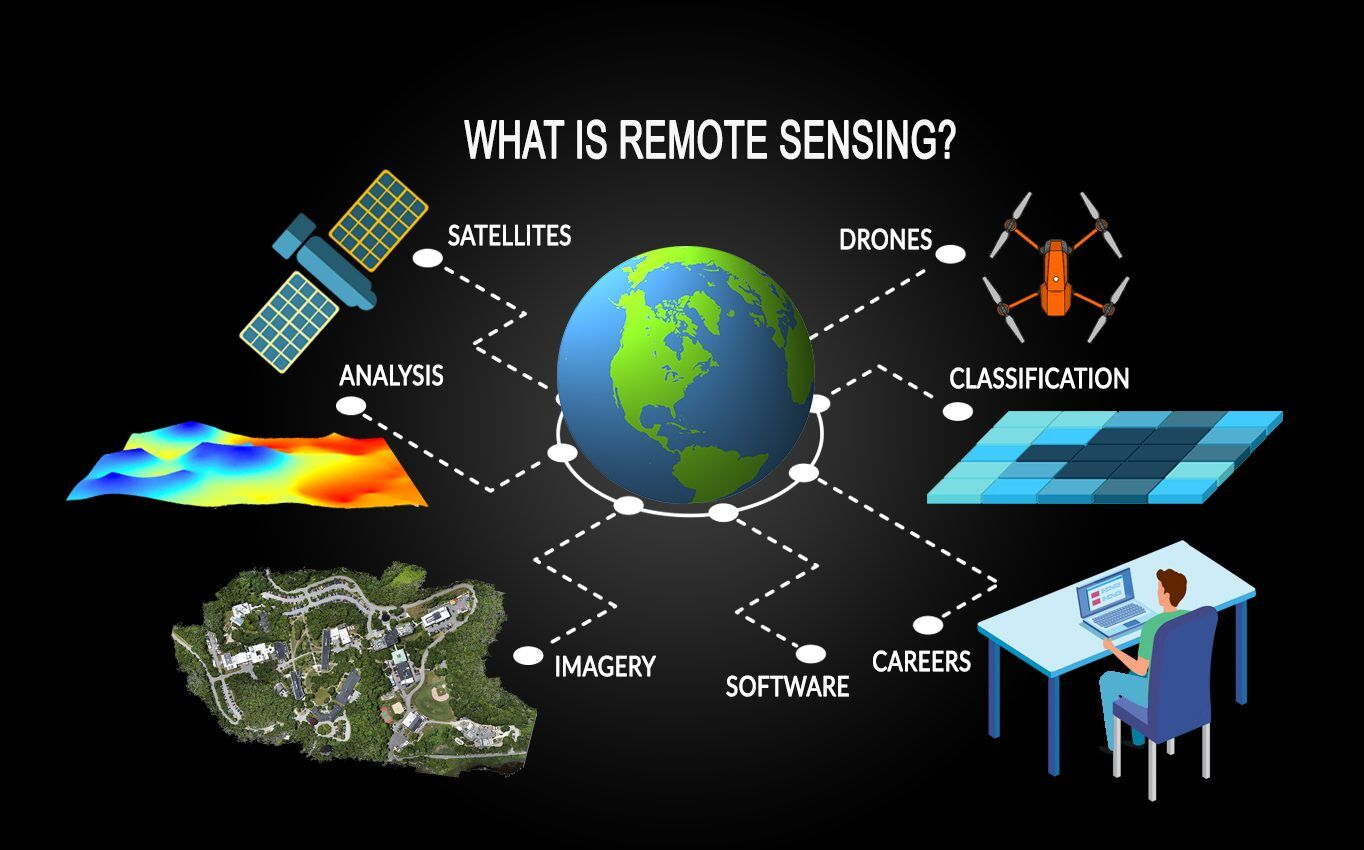
\includegraphics{./image/remote.jpg}

}

\caption{What is Remote Sensing}

\end{figure}

\bookmarksetup{startatroot}

\hypertarget{sec-week1-getting-started-with-remote-sensing}{%
\chapter{Week1: Getting started with remote
sensing}\label{sec-week1-getting-started-with-remote-sensing}}

\hypertarget{summary}{%
\section{Summary}\label{summary}}

\hypertarget{the-concept-of-remote-sensing}{%
\subsection{The concept of remote
sensing}\label{the-concept-of-remote-sensing}}

In contrast to in situ or on-site observation, remote sensing is the
process of gathering data about a phenomenon or object without actually
coming into touch with it. The phrase is used particularly in reference
to learning more about Earth and other planets.

The phrase ``remote sensing'' today typically refers to the detection
and classification of Earthly objects using satellite- or aircraft-based
sensor technologies. Based on transmitted signals, it encompasses the
atmosphere, the surface, and the oceans (e.g.~electromagnetic
radiation). It can be divided into ``active'' and ``passive'' remote
sensing (where a signal is emitted to the object by a satellite or
aircraft and its reflection is detected by the sensor) (when the
reflection of sunlight is detected by the sensor)

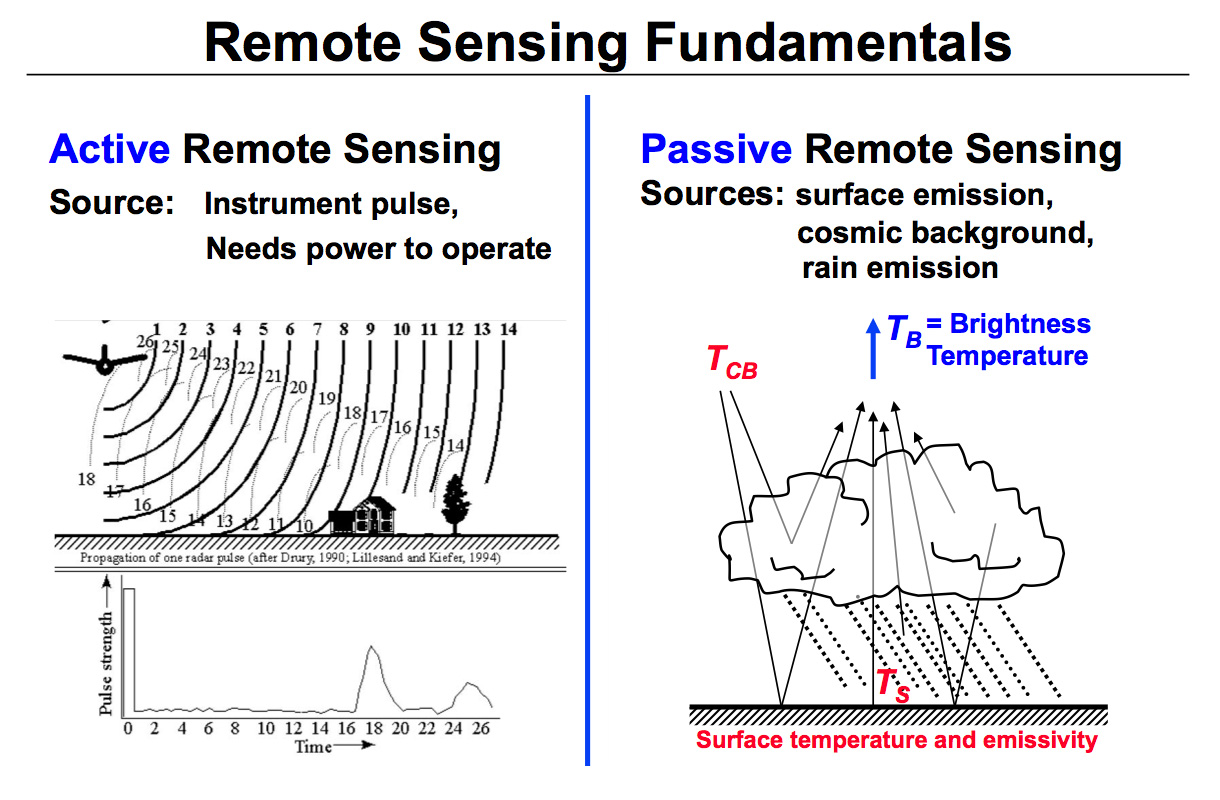
\includegraphics{./image/diagram.jpg}

\hypertarget{piece-of-work}{%
\subsection{Piece of work:}\label{piece-of-work}}

In the first chapter, I learned how to access remote sensing data using
two open source databases, Landsat and Copernicus Open Access Hub, their
existence make it easy for me to access remote sensing data from
anywhere in the world.

Secondly, I learned how to use QGIS, SNAP and some packages in R for
simple raster processing calculations. I used my own case and followed
the instructions step by step, learning a lot about the terminology,
gaining some knowledge about remote sensing and statistics and also
having some questions.

\hypertarget{application}{%
\section{Application}\label{application}}

\hypertarget{qgis}{%
\subsection{QGIS}\label{qgis}}

When learning QGIS, I used as an example a map of Zhenjiang and
Changzhou, two cities in Jiangsu Province, China, bordered by the
Yangtze River to the north, from Copernicus Open Access Hub. Then,
merged the B2 (blue), B3 (green), B4 (red) and B8 (NIR) in R10m with
multiband colour, and knew the details in different enhancement options.
Then, I learned about difference between R10m and R20m. Generally,
upsampling is used to complement the situation when the pixel resolution
is greater than the source resolution, and a common interpolation method
is nearest neighbour, while downsampling is used when pixel resolution
is smaller than source resolution. Here is the mechanism of nearest
neighbour:

\(X_{src}=X_{dst}*\frac{Width_{src}}{Width_{dst}}\)

\(Y_{src}=Y_{dst}*\frac{Height_{src}}{Height_{dst}}\)

If the calculation results in a fractional number, then either remove
the decimal part or round up to get the same value as the original
dotted pixel. This method is very simple but inaccurate, the zoomed in
image has a very bad mosaic and the zoomed out image has a very bad
distortion. The problem lies in the treatment of the fractional part,
which is equivalent to the process of colour gradation and cannot be
fully equated with the existing colour of pixel. It is possible to use
bilinear interpolation, considering the four values around the point
that needs to be scaled, to see which value has more influence on it,
and to give it more weight, I saw the option of bilinear interpolation
then tried it. In addition, cubic has more accurate result because
non-linear function can fit better but more complex.

\hypertarget{snap}{%
\subsection{SNAP}\label{snap}}

The sRBG standard colour space can be used for display, network
transmission and to convert colour levels on other devices into a colour
space that is recognisable to the computer by means of the sRGB
conversion function. This is why the brightness levels in the range
{[}0,4095{]} on the Sentinel-2 can be converted to values in the range
{[}0,255{]}.

When using SNAP, 432 nm means this wavelength is 432 nm, it is a coastal
aerosol wave which wavelength is lessmthan blue wave. I like the colour
composition function, which allows me to highlight different sections
depending on my needs.

\begin{figure}

{\centering 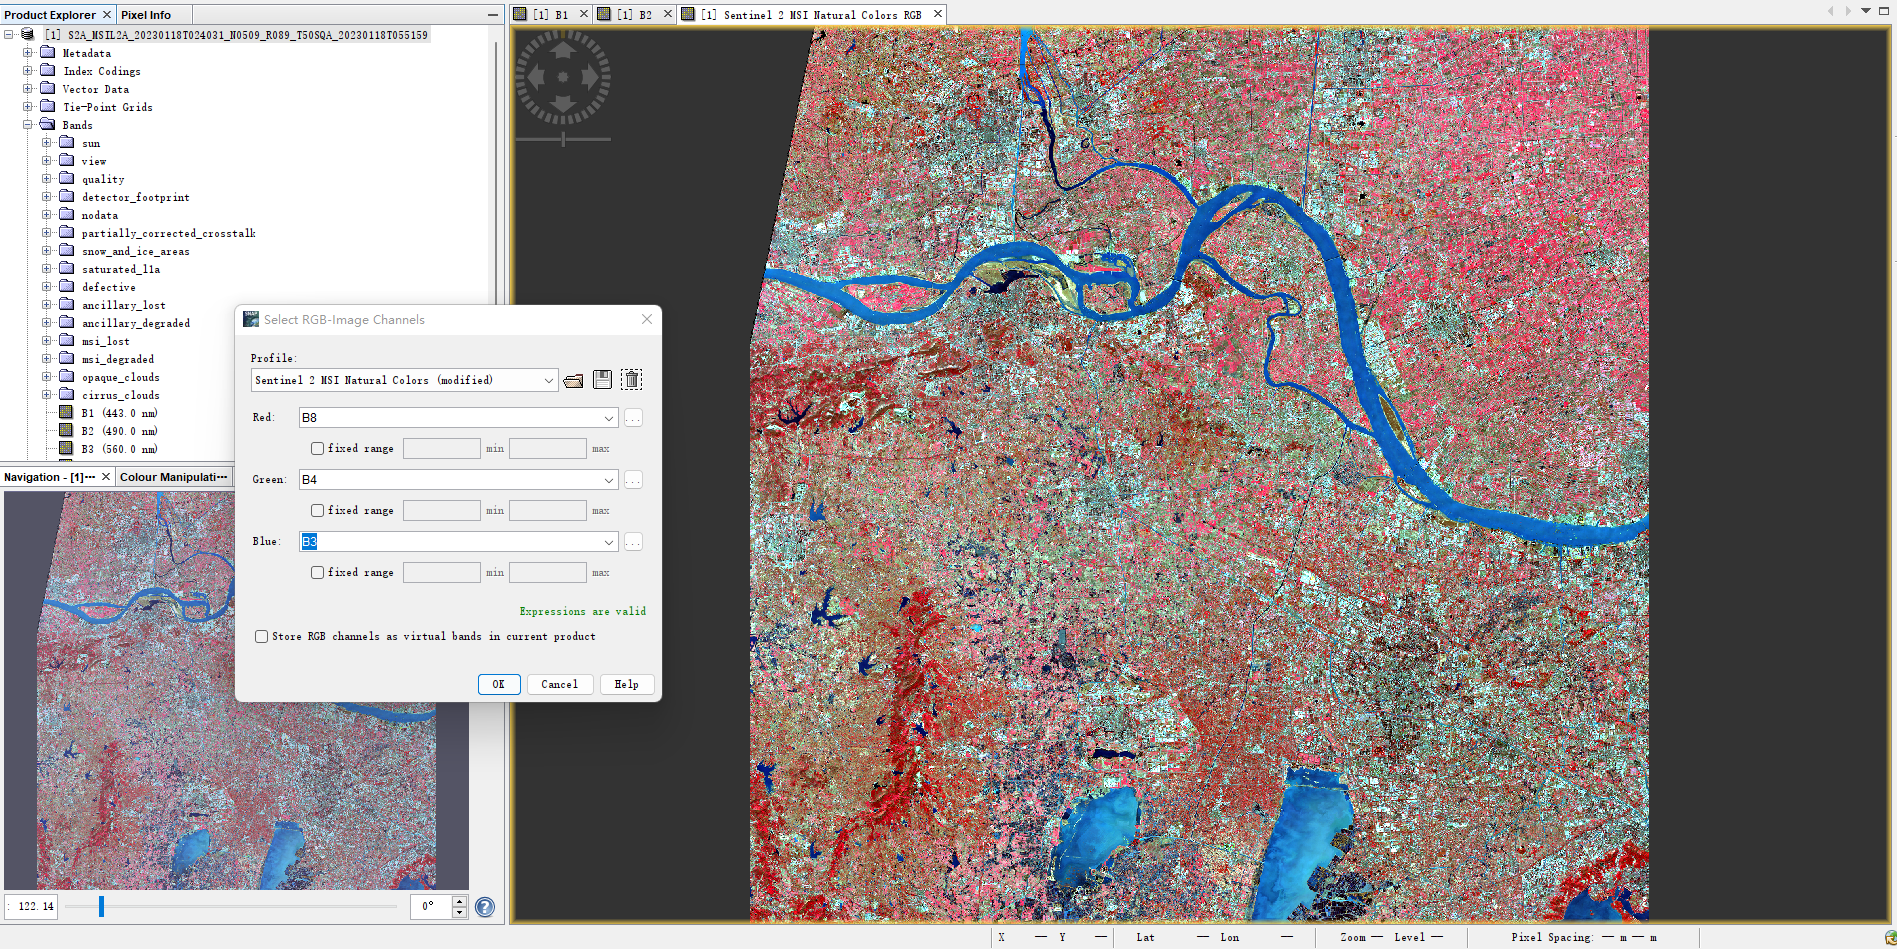
\includegraphics[width=6.25in,height=\textheight]{./image/B8-B4-B3.png}

}

\caption{B8-B4-B3}

\end{figure}

Here is the scatter plot of my example:

\begin{figure}

{\centering 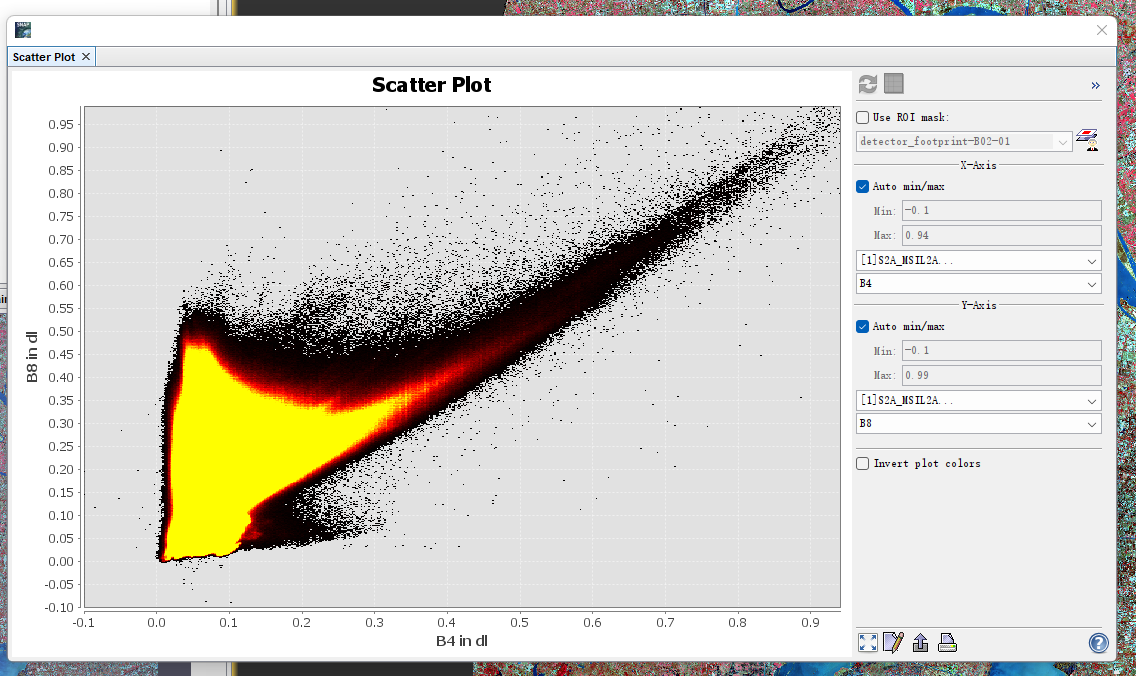
\includegraphics[width=6.25in,height=\textheight]{./image/scatterplot.png}

}

\caption{scatterplot}

\end{figure}

It can be seen that map of Zhenjiang and Changzhou has high brightness
level, which means it is a city area, and it also shows a lot of wet
bare soil, we can assume that these wet soils may be more suitable for
cultivation, the overall biomass is not very large and, most notably,
there is also a lot of dry bare soil lack of vegetation cover,
presumably non-agricultural land.

When using mask function, I got the administrative divisions of these
municipalities because I downloaded the administrative divisions of
China from GADM data:

\begin{figure}

{\centering 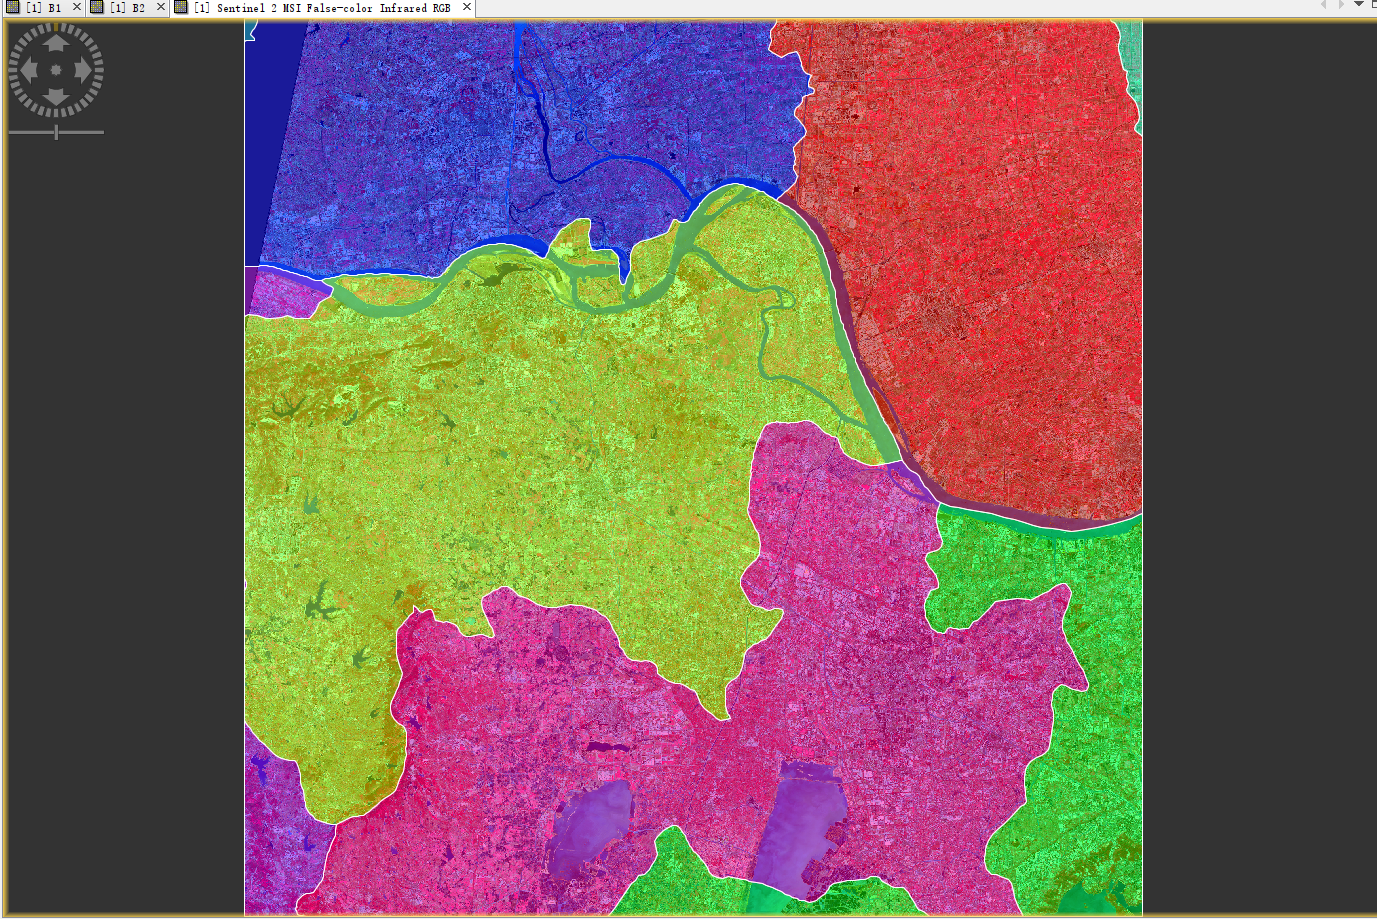
\includegraphics[width=6.25in,height=\textheight]{./image/citys.png}

}

\caption{administrative divisions}

\end{figure}

(yellow: Zhenjiang, pink:Changzhou, red: Taizhou, green:Wuxi, blue:
Yangzhou)

After resampling and downscaling the data I got this tasselled plot,
compared to the previous one I found that the downscaling had reduced
the urban part, so the plot was significantly less bright, and there was
more wet bare soil present than the previous one.

\begin{figure}

{\centering 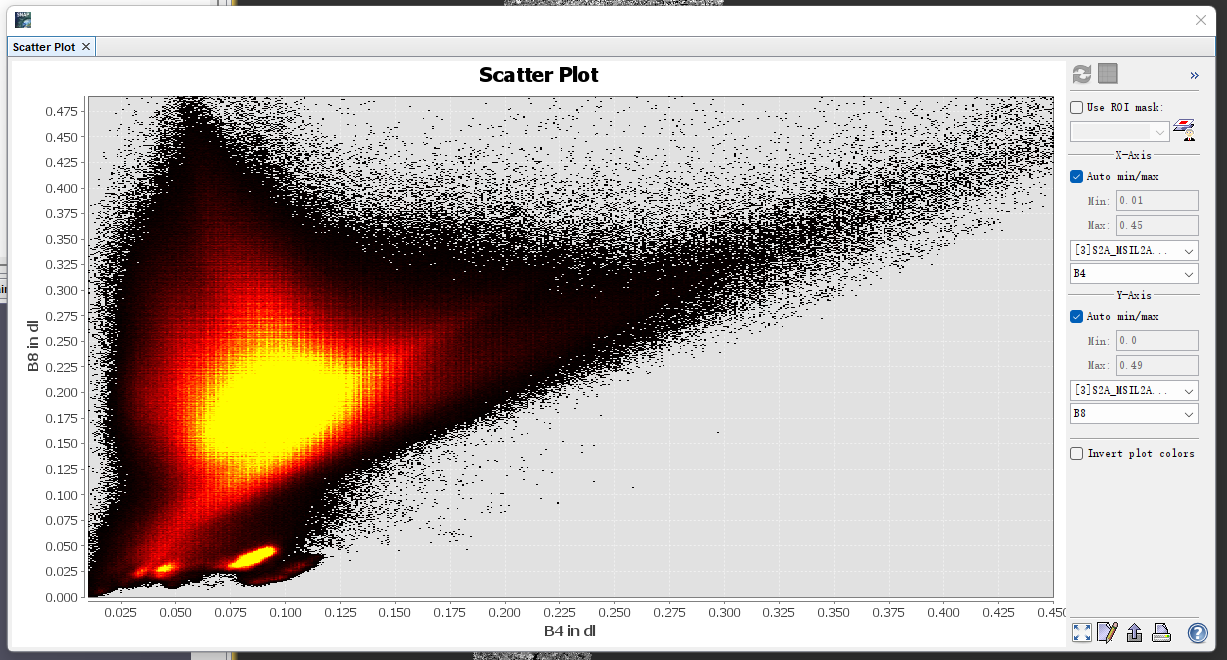
\includegraphics[width=6.25in,height=\textheight]{./image/scatterplot2.png}

}

\caption{scatterplot}

\end{figure}

Generally speaking, I prefer using SNAP than QGIS because it has more
vivid chart and we can evaluate the local soil conditions, the size of
the city and the biomass.

\hypertarget{r-script}{%
\subsection{R script}\label{r-script}}

When learning the code to deal with data from Landsat and Sentinel, I
found a final paired t-test is performed to test whether the actual
means of the urban land type from Landsat and Sentinel are equal, the
degree of freedom from the results is 5970, p-value is much smaller than
0.05, which means the actual means of two groups are quite different,
and at the same time, this calculation also shows the estimate mean of
two samples. There are 95\% probability that the true mean is between
-9300.307 and -9198.368. data from Sentinel and Landsat is different.

\hypertarget{reflection}{%
\section{Reflection}\label{reflection}}

Remote sensing technology is now widely used in scientific research and
practice, for land planning, geological exploration and forest fire
prevention, so learning to make remote sensing maps is an essential
skill.

There are several areas of interest to me, one of them is how PCA can be
used to reduce the dimensionality of data, particularly in image
processing, and I will be doing further study and figuring this out.
Then, I would like to know if the image data from satellite remote
sensing can be used in AI, as there are already mature deep learning
algorithms with a high accuracy rate for image recognition, how to use
these images to achieve functions such as automatic recognition and
automatic monitoring.

\bookmarksetup{startatroot}

\hypertarget{week2-portfolio}{%
\chapter{Week2: Portfolio}\label{week2-portfolio}}

Here is the link of presentation which is created via Xaringan:
https://GIScodingMo.github.io/week2\_xaringan

\bookmarksetup{startatroot}

\hypertarget{references}{%
\chapter*{References}\label{references}}
\addcontentsline{toc}{chapter}{References}

\markboth{References}{References}

\hypertarget{refs}{}
\begin{CSLReferences}{0}{0}
\end{CSLReferences}



\end{document}
